%% This is an example first chapter.  You should put chapter/appendix that you
%% write into a separate file, and add a line \include{yourfilename} to
%% main.tex, where `yourfilename.tex' is the name of the chapter/appendix file.
%% You can process specific files by typing their names in at the 
%% \files=
%% prompt when you run the file main.tex through LaTeX.
\chapter{Introduction}

Recent years have seen a rise in cybersecurity attacks. From the 2016 Democratic National Committee (DNC) hack \cite{dnc-hack} to the WannaCry ransomware attack on the U.K. National Health Service \cite{wannacry-uk}, effects of these attacks can range from influencing elections to disrupting health care throughout the country. As more of the world moves towards online systems, the attackers are increasingly motivated to try newer and more sophisticated attacks.

On the opposing end, there have been developments in the cybersecurity front as well. Most products release regular security updates to fix bugs in their software. However, very few focus on the heart of these attacks - phishing attacks. A recent report \cite{phishme-report} published by PhishMe, a phishing defense solutions company, in 2016 found that ``91\% of cyberattacks and resulting data breach begin with a spear phishing email'' \cite{91phishing}.

\section{Phishing Attacks}

A \textit{phishing attack} is a type of attack intended to trick the user into revealing sensitive information for malicious purposes. Such an attack is commonly executed through fake emails or websites.  A successful phishing attack may steal user credentials or install malicious software on their system, eventually leaving the user open to other forms of attacks.

\begin{figure}[p]
\centering
    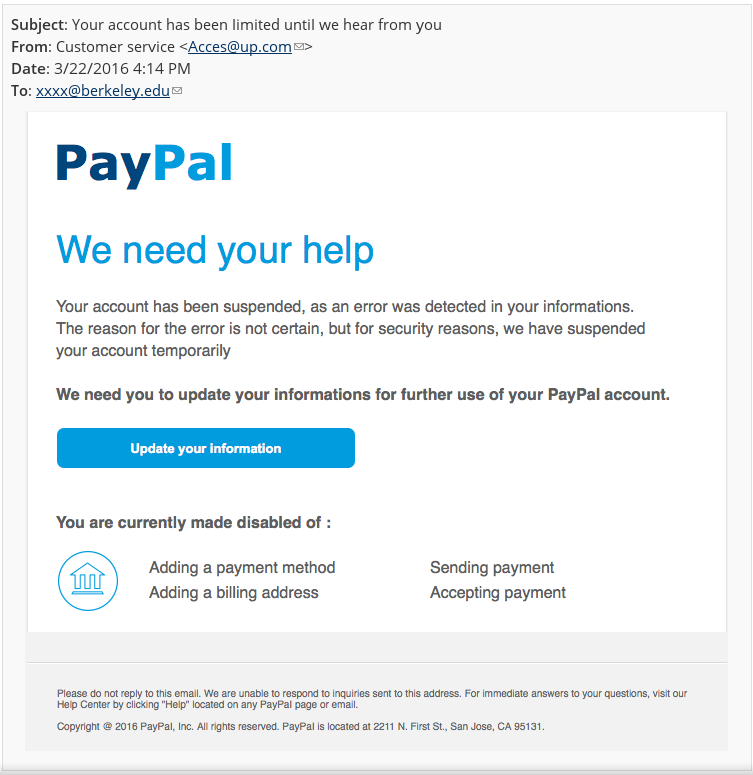
\includegraphics[width=1.0\textwidth]{phishing_example_paypal.png}
    \caption{This figure shows a phishing email disguised to appear to come from Paypal. The link shown in the email leads to a fake login page which allows the attacker to steal user credentials.}
   \label{fig:phishing-example-paypal}
\end{figure}
\begin{figure}[p]
\centering
    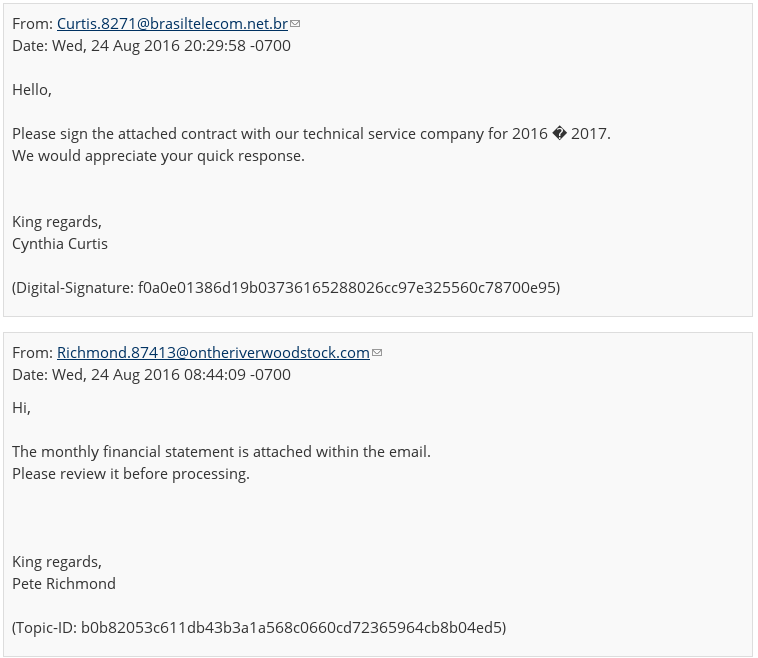
\includegraphics[width=1.0\textwidth]{phishing_example_malware.png}
    \caption{This figure shows a phishing email with an attachment that, when executed, installs a ransomware onto the user's computer.}
   \label{fig:phishing-example-malware}
\end{figure}

Figure \ref{fig:phishing-example-paypal} shows a phishing email \cite{phishing-example-paypal} that appears to originate from Paypal, an online money transaction service. It asks the user to click on a link to update their information. Upon clicking, the user is redirected to a fake Paypal login page intended to steal the user's credentials.

Figure \ref{fig:phishing-example-malware} shows a phishing email \cite{phishing-example-malware} with an attachment that appears to contain the user's monthly financial statement or a service contract. The attachment is a malicious file which, upon execution, encrypts all the files on the computer and shows a ransom message on the screen.

As recent attacks have demonstrated, current systems do not take sufficient measures to protect users from phishing attacks. Such attacks may take place through various methods and are hard to defend against. In most cases, users are either not careful enough, or are unaware of the expectations from genuine sources. Therefore, they miss the cues that tells them that a phishing attack is taking place. This thesis presents the design of \namesecureworkstation/, a workstation to better defend against cyberattacks, specifically phishing attacks.

\section{Approach}

\namesecureworkstation/ is composed of three parts: (i) Qubes OS, a virtualization-based operating system that provides strong isolation guarantees, (ii) a HTTP/HTTPS proxy filter that uses the technique of deep packet inspection \cite{deep-packet-inspection}, (iii) a secure and unambiguous user interface for browsing the web, and (iv) a filtering policy called Site Aggregate Isolation.

The goal of Quboid is to defend against phishing sources, specifically phishing attempts which occur through user-created content such as public forums, instant messaging, emails, etc. We introduce a new filtering policy called Site Aggregate Isolation. The policy dictates that websites with logically unrelated content must not share state and should not be able to communicate with each other. For example, Gmail and Bank of America are different products and should be isolated whereas Facebook Web and Messenger may be allowed to share state. Current systems lack the mechanism to reliably identify which website is being displayed to the user. Phishing attacks take advantage of this to trick the user into trusting the phishing content to be genuine. We believe that the policies introduced in this thesis will help reducing this ambiguity and thus provide stronger guarantees for preventing phishing attacks.

\namesecureworkstation/ implements the Site Aggregate Isolation policy in two places. Firstly, it uses separate browser instances to isolate websites belonging to different site-aggregates, a group of related websites. It uses Qubes OS \cite{qubes-os}, an operating system that uses virtualization for isolation, to run each browser instance in an isolated virtual machine. This ensures that no state can be shared between different site-aggregates. This also ensures that in the event one browser instance gets compromised, the damage is limited to just that virtual machine.
Secondly, traffic from each virtual machine is routed through an intermediate proxy VM. The proxy VM is responsible for filtering requests and enforcing the rest of the Site Aggregate Isolation policy.

For security in user interaction, \namesecureworkstation/ also contains of a secure user interface. The interface consists of a single application window manager restricted to displaying only one browser instance on the screen at anytime. A part of the screen is reserved exclusively for showing the site-aggregate name of the active browser instance. We believe these steps help prevent phishing attacks by reducing the ambiguity of the user interface.

\section{Contributions}

This thesis introduces a set of new policies. These policies allow a safer browsing experience with some loss of usability. The policy design includes the following:

\begin{itemize}
    \item a website identification and isolation mechanism called \textit{Site Aggregate Isolation},
    \item exceptions to this policy to allow websites to refer to external resources and communicate with websites belonging to other site-aggregates, and
    \item guidelines for the interface of the browsing client to reduce the ambiguity regarding the site-aggregate name of the content shown on the screen.
\end{itemize}

This thesis also presents an implementation of these policies in the form of a workstation. The implementation includes the following:

\begin{itemize}
    \item \namesecureworkstation/, a system developed on top of Qubes OS to open browser instances belonging to different site-aggregates in separate virtual machines,
    \item set of HTTP response headers that include additional information such as the site-aggregate name of the website, set of external resources needed, etc., and
    \item a secure user interface with reserved areas for the system and the applications, and a clear display of the site-aggregate name of the currently active browser instance.
\end{itemize}

It is difficult to ensure that no malicious content is encountered by a user while browsing the web. The principal contribution of \namesecureworkstation/ is an increased awareness in the ability of the user to identify malicious content and safely browse the web without any harmful effects.

\paragraph{Limitations:} A major part of our proposed system requires changes in the structure of existing websites. Quboid introduces a number of HTTP header fields in our design. Since these are new header fields, current websites will have to include them in their implementation. Furthermore, a possible misconfiguration by website developers may still leave the users vulnerable to phishing attacks.

\namesecureworkstation/ defends against some but not all forms of phishing attacks. Although the system takes several steps to reduce the possibility of a successful attack, the security of the system still rests in the hands of the user. The interface provides cues to the user when there is a possibility of a phishing attack. If the user is not careful enough to recognize them, they may still fall victim to phishing attacks.

The everyday browsing experience of the user is also changed. Quboid offers strict isolation when browsing the web. This means if users want to download a new software, it will also be run in an isolated virtual machine. The system does not provide an easy way to interact with other software running in different virtual machines.

\section{Outline of thesis}

Chapter~\ref{chap:relatedwork} describes related work regarding creating secure workstations. We analyze the different approaches taken by modern-day systems, ranging from a full-blown operating system to methods like spam filters in email clients. We begin by describing the different ways phishing attacks operate, followed by analyzing each system to see where they fail in defending against such attacks.

Chapter~\ref{chap:goals} describes the goals of this thesis. We list properties a secure workstation must have to prevent phishing attacks. Additionally, we give examples of phishing attacks to justify the importance of these properties. We emphasize a secure workstation's ability to block malicious content, present an unambiguous user interface, and contain damage in the event of a breach.

Chapter~\ref{chap:design} describes the design of the workstation proposed in this thesis. We describe in detail new policies targeted at attacks originating from user-created content. We also describe ways to implement these policies in a proxy filter using the technique of deep packet inspection.

Chapter~\ref{chap:implementation} gives the implementation details of \namesecureworkstation/. We describe the different subsystems used and the pros and cons of some alternate implementations of these subsystems.

Chapter~\ref{chap:analysis} analyzes the effectiveness of the system as a whole in defending against recent real-world phishing attacks and various fictional phishing scenarios. Of course, our system does not defend against all forms of foreseeable attacks, however, it is able to defend against a majority of attacks that current systems do not.

Chapter~\ref{chap:conclusion} concludes this thesis with a summary of \namesecureworkstation/. A majority of cyberattacks start off with a phishing attack on an unsuspecting user. The secure workstation developed focuses on the heart of the methods used in these cyberattacks. Our hope is that with this workstation, users are able to browse the internet without worrying about downloading unsolicited software from unknown websites or having their details unsuspectingly stolen during day-to-day browsing.